\documentclass[a4paper]{article}
\usepackage{vntex}
%\usepackage[english,vietnam]{babel}
%\usepackage[utf8]{inputenc}
\usepackage{float}
%\usepackage[utf8]{inputenc}
%\usepackage[francais]{babel}
\usepackage{a4wide,amssymb,epsfig,latexsym,multicol,array,hhline,fancyhdr}
\usepackage{booktabs}
\usepackage{amsmath}
\usepackage{lastpage}
\usepackage[lined,boxed,commentsnumbered]{algorithm2e}
\usepackage{enumerate}
\usepackage{color}
\usepackage{graphicx}							% Standard graphics package
\usepackage{array}
\usepackage{tabularx, caption}
\usepackage{multirow}
\usepackage[framemethod=tikz]{mdframed}% For highlighting paragraph backgrounds
\usepackage{multicol}
\usepackage{rotating}
\usepackage{graphics}
\usepackage{geometry}
\usepackage{setspace}
\usepackage{epsfig}
\usepackage{tikz}
\usepackage{listings}
\usepackage{longtable}
\usepackage{xcolor}
\usepackage{colortbl}
\usetikzlibrary{arrows,snakes,backgrounds}
\usepackage{hyperref}
\hypersetup{urlcolor=blue,linkcolor=black,citecolor=black,colorlinks=true}
%\usepackage{pstcol} 								% PSTricks with the standard color package

\newtheorem{theorem}{{\bf Định lý}}
\newtheorem{property}{{\bf Tính chất}}
\newtheorem{proposition}{{\bf Mệnh đề}}
\newtheorem{corollary}[proposition]{{\bf Hệ quả}}
\newtheorem{lemma}[proposition]{{\bf Bổ đề}}

\everymath{\color{blue}}
%\usepackage{fancyhdr}
\setlength{\headheight}{40pt}
\pagestyle{fancy}
\fancyhead{} % clear all header fields
\fancyhead[L]{
 \begin{tabular}{rl}
    \begin{picture}(25,15)(0,0)
    \put(0,-8){\includegraphics[width=8mm, height=8mm]{logoITSGUsmall.png}}
    %\put(0,-8){\epsfig{width=10mm,figure=hcmut.eps}}
   \end{picture}&
	%\includegraphics[width=8mm, height=8mm]{hcmut.png} & %
	\begin{tabular}{l}
		\textbf{\bf \ttfamily Trường Đại học Sài Gòn}\\
		\textbf{\bf \ttfamily Khoa Công Nghệ Thông Tin}
	\end{tabular}
 \end{tabular}
}
\fancyhead[R]{
	\begin{tabular}{l}
		\tiny \bf \\
		\tiny \bf
	\end{tabular}  }
\fancyfoot{} % clear all footer fields
\fancyfoot[L]{\scriptsize \ttfamily Bài tập lớn môn Ngôn ngữ lập trình C\# - Niên khóa 2025-2026}
\fancyfoot[R]{\scriptsize \ttfamily Trang {\thepage}/\pageref{LastPage}}
\renewcommand{\headrulewidth}{0.3pt}
\renewcommand{\footrulewidth}{0.3pt}


%%%
\setcounter{secnumdepth}{4}
\setcounter{tocdepth}{3}
\makeatletter
\newcounter {subsubsubsection}[subsubsection]
\renewcommand\thesubsubsubsection{\thesubsubsection .\@alph\c@subsubsubsection}
\newcommand\subsubsubsection{\@startsection{subsubsubsection}{4}{\z@}%
                                     {-3.25ex\@plus -1ex \@minus -.2ex}%
                                     {1.5ex \@plus .2ex}%
                                     {\normalfont\normalsize\bfseries}}
\newcommand*\l@subsubsubsection{\@dottedtocline{3}{10.0em}{4.1em}}
\newcommand*{\subsubsubsectionmark}[1]{}
\makeatother

\definecolor{dkgreen}{rgb}{0,0.6,0}
\definecolor{gray}{rgb}{0.5,0.5,0.5}
\definecolor{mauve}{rgb}{0.58,0,0.82}
\definecolor{headerblue}{RGB}{30,80,160}
\definecolor{rowgray}{RGB}{245,246,248}

\lstset{frame=tb,
	language=Matlab,
	aboveskip=3mm,
	belowskip=3mm,
	showstringspaces=false,
	columns=flexible,
	basicstyle={\small\ttfamily},
	numbers=none,
	numberstyle=\tiny\color{gray},
	keywordstyle=\color{blue},
	commentstyle=\color{dkgreen},
	stringstyle=\color{mauve},
	breaklines=true,
	breakatwhitespace=true,
	tabsize=3,
	numbers=left,
	stepnumber=1,
	numbersep=1pt,
	firstnumber=1,
	numberfirstline=true
}

% Kiểu cột tiện dụng cho longtable
\newcolumntype{L}[1]{>{\raggedright\arraybackslash}p{#1}}
\newcolumntype{C}[1]{>{\centering\arraybackslash}p{#1}}

\begin{document}

\begin{titlepage}
\begin{center}
TRƯỜNG ĐẠI HỌC SÀI GÒN \\
KHOA CÔNG NGHỆ THÔNG TIN
\end{center}
\vspace{1cm}

\begin{figure}[h!]
\begin{center}
\includegraphics[width=3cm]{logoITSGU.png}
\end{center}
\end{figure}

\vspace{1cm}


\begin{center}
\begin{tabular}{c}
	\multicolumn{1}{l}{\textbf{{\Large NGÔN NGỮ LẬP TRÌNH C\#}}}\\
	~~\\
	\hline
	\\
	\multicolumn{1}{l}{\textbf{{\Large Xử lý bài toán }}}\\
	\\

	\textbf{{\Huge Ứng dụng mạng xã hội Instory}}\\
	\\
	\hline
\end{tabular}
\end{center}

\vspace{3cm}

\begin{table}[h]
\begin{tabular}{rrl}
\hspace{5 cm} & GVHD: &Từ Lãng Phiêu\\
& SV: & Hồ Quốc Bảo - 3123410016\\
& & Trần Minh Đăng - 3123410078 \\
& & Bùi Nguyễn Trọng Nghĩa - 3123560052 \\
& & Lê Thị Khánh Linh - 3124410187 \\
& & Nguyễn Thị Loan - 3124410191 \\

\end{tabular}
\vspace{1.5 cm}
\end{table}

\begin{center}

{\footnotesize TP. HỒ CHÍ MINH, THÁNG 5/2026}
\end{center}
\end{titlepage}


\thispagestyle{empty}

\newpage
\tableofcontents
\newpage

%%%%%%%%%%%%%%%%%%%%%%%%%%%%%%%%%
%%%%%%%%%%%%%%%%%%%%%%%%%%%%%%%%%
% PHẦN 1: THIẾT KẾ CƠ SỞ DỮ LIỆU
%%%%%%%%%%%%%%%%%%%%%%%%%%%%%%%%%
\newpage
\section{Thiết kế Cơ sở Dữ liệu (ERD)}
Hệ thống sử dụng cơ sở dữ liệu quan hệ để quản lý các thực thể người dùng, tương tác mạng xã hội và tin nhắn thời gian thực. Dưới đây là cấu trúc chi tiết được chia thành các phân vùng chức năng:

\subsection{Quản lý Người dùng và Quan hệ}
Phần này tập trung vào thực thể người dùng (tích hợp [ASP.NET](http://ASP.NET) Identity) và các mối quan hệ bạn bè, theo dõi.
\begin{figure}[H]
	\begin{center}
		\includegraphics[width=0.85\textwidth]{image/ERD1.png}
		\caption{Sơ đồ ERD - Quản lý người dùng và quan hệ}
	\end{center}
\end{figure}

\subsection{Quản lý Bài viết và Tương tác}
Bao gồm các bảng lưu trữ bài viết, hình ảnh đi kèm, lượt thích, bình luận và báo cáo nội dung.
\begin{figure}[H]
	\begin{center}
		\includegraphics[width=0.85\textwidth]{image/ERD2.png}
		\caption{Sơ đồ ERD - Quản lý bài viết và tương tác}
	\end{center}
\end{figure}

\subsection{Quản lý Tin nhắn và Story}
Cấu trúc cho phép lưu trữ tin nhắn trong các cuộc hội thoại và các tin đăng tạm thời (Story).
\begin{figure}[H]
	\begin{center}
		\includegraphics[width=0.85\textwidth]{image/ERD3.png}
		\caption{Sơ đồ ERD - Hệ thống Chat và Story}
	\end{center}
\end{figure}

%%%%%%%%%%%%%%%%%%%%%%%%%%%%%%%%%
% PHẦN 2: LUỒNG CHỨC NĂNG (FLOWCHART)
%%%%%%%%%%%%%%%%%%%%%%%%%%%%%%%%%
\newpage
\section{Luồng nghiệp vụ của các chức năng chính}

\subsection{Chức năng Đăng ký tài khoản (Sign-up)}
Quy trình đảm bảo tính xác thực bằng cách sử dụng mã OTP gửi qua Email trước khi khởi tạo tài khoản chính thức.
\begin{figure}[H]
	\begin{center}
		\includegraphics[width=0.7\textwidth]{image/signup_flowchart.png}
		\caption{Flowchart quy trình đăng ký và xác thực OTP}
	\end{center}
\end{figure}

\subsection{Chức năng Đăng nhập (Login)}
Hệ thống hỗ trợ đăng nhập truyền thống qua mật khẩu và đăng nhập nhanh qua bên thứ ba (Google).
    \begin{figure}[H]
		\centering
		\includegraphics[width=0.45\textwidth]{image/login_flowchart.png}
		\caption{Flowchart đăng nhập truyền thống}
	\end{figure}
	\begin{figure}[H]
		\centering
		\includegraphics[width=0.45\textwidth]{image/google_login_flowchart.png}
		\caption{Flowchart đăng nhập Google}
	\end{figure}

\subsection{Chức năng Nhắn tin thời gian thực (Chat)}
Sử dụng công nghệ SignalR để đảm bảo tin nhắn được truyền tải tức thời giữa các bên.
\begin{figure}[H]
	\begin{center}
		\includegraphics[width=0.6\textwidth]{image/chat_flowchart.png}
		\caption{Flowchart quy trình nhắn tin thời gian thực}
	\end{center}
\end{figure}

\subsection{Chức năng Quản lý bài viết (Post Management)}
\subsubsection{Tạo bài viết (Create Post)}
\begin{figure}[H]
	\begin{center}
		\includegraphics[width=1\textwidth]{image/createpost_flowchart.png}
		\caption{Flowchart quy trình tạo bài viết}
	\end{center}
\end{figure}

\subsubsection{Cập nhật bài viết (Update Post)}
\begin{figure}[H]
	\begin{center}
		\includegraphics[width=1.2\textwidth]{image/updatepost_flowchart.png}
		\caption{Flowchart quy trình cập nhật bài viết}
	\end{center}
\end{figure}

\subsubsection{Xóa bài viết (Delete Post)}
\begin{figure}[H]
	\begin{center}
		\includegraphics[width=0.6\textwidth]{image/deletepost_flowchart.png}
		\caption{Flowchart quy trình xóa bài viết}
	\end{center}
\end{figure}

\subsection{Chức năng Tương tác bài viết (Post Interaction)}
\subsubsection{Thích/Bỏ thích (Like/Unlike)}
\begin{figure}[H]
	\begin{center}
		\includegraphics[width=0.6\textwidth]{image/likepost_flowchart.png}
		\caption{Flowchart quy trình thích/bỏ thích bài viết}
	\end{center}
\end{figure}

\subsubsection{Bình luận (Comment)}
\begin{figure}[H]
	\begin{center}
		\includegraphics[width=0.6\textwidth]{image/commentpost_flowchart.png}
		\caption{Flowchart quy trình bình luận bài viết}
	\end{center}
\end{figure}

\subsubsection{Chia sẻ (Share)}
\begin{figure}[H]
	\begin{center}
		\includegraphics[width=0.6\textwidth]{image/sharepost_flowchart.png}
		\caption{Flowchart quy trình chia sẻ bài viết}
	\end{center}
\end{figure}

\subsubsection{Báo cáo (Report)}
\begin{figure}[H]
	\begin{center}
		\includegraphics[width=0.6\textwidth]{image/reportpost_flowchart.png}
		\caption{Flowchart quy trình báo cáo bài viết}
	\end{center}
\end{figure}

%---------------------------------------------------------------------
\subsection{Chức năng Story}
Story là nội dung ảnh tạm thời, tự hết hạn sau 24 giờ. Người dùng có thể tạo, xem và xóa story của mình.

\subsubsection{Tạo Story (Create Story)}
Người dùng upload ảnh (JPEG, PNG, WebP, GIF, tối đa 10 MB); hệ thống từ chối video và các định dạng không được hỗ trợ trước khi lưu lên S3.
\begin{figure}[H]
	\begin{center}
		\includegraphics[width=0.65\textwidth]{image/createstory_flowchart.png}
		\caption{Flowchart quy trình tạo Story}
	\end{center}
\end{figure}

\subsubsection{Xem Story (View Story)}
Khi một người dùng mở story của người khác, hệ thống ghi nhận lượt xem. Cơ chế này là idempotent: gọi nhiều lần cho cùng một cặp (story, viewer) chỉ tạo một bản ghi duy nhất.
\begin{figure}[H]
	\begin{center}
		\includegraphics[width=0.6\textwidth]{image/viewstory_flowchart.png}
		\caption{Flowchart quy trình xem Story}
	\end{center}
\end{figure}

\subsubsection{Xóa Story (Delete Story)}
Chỉ chủ sở hữu mới có thể xóa. Hệ thống xóa bản ghi DB trước, sau đó mới xóa file trên S3 để tránh mất dữ liệu nếu thao tác S3 thất bại.
\begin{figure}[H]
	\begin{center}
		\includegraphics[width=0.6\textwidth]{image/deletestory_flowchart.png}
		\caption{Flowchart quy trình xóa Story}
	\end{center}
\end{figure}

%---------------------------------------------------------------------
\subsection{Chức năng Highlight}
Highlight cho phép người dùng lưu trữ vĩnh viễn các Story đã hết hạn thành các bộ sưu tập có tiêu đề. Ảnh bìa được sao chép độc lập trên S3 để tránh bị ảnh hưởng khi story gốc bị xóa.

\subsubsection{Tạo Highlight (Create Highlight)}
\begin{figure}[H]
	\begin{center}
		\includegraphics[width=0.65\textwidth]{image/createhighlight_flowchart.png}
		\caption{Flowchart quy trình tạo Highlight}
	\end{center}
\end{figure}

\subsubsection{Thêm / Xóa Story khỏi Highlight}
\begin{figure}[H]
	\begin{center}
		\includegraphics[width=0.65\textwidth]{image/highlightstory_flowchart.png}
		\caption{Flowchart quy trình thêm/xóa Story trong Highlight}
	\end{center}
\end{figure}

\subsubsection{Xóa Highlight (Delete Highlight)}
\begin{figure}[H]
	\begin{center}
		\includegraphics[width=0.55\textwidth]{image/deletehighlight_flowchart.png}
		\caption{Flowchart quy trình xóa Highlight}
	\end{center}
\end{figure}

%---------------------------------------------------------------------
\subsection{Chức năng Kết bạn (Follow / Friendship)}
Instory dùng mô hình kết bạn hai chiều (friendship): người dùng gửi lời mời, người nhận chấp nhận hoặc từ chối. Khi chấp nhận, hệ thống tự động tạo cuộc trò chuyện riêng (Direct Chat) giữa hai người.

\subsubsection{Gửi / Hủy lời mời kết bạn}
\begin{figure}[H]
	\begin{center}
		\includegraphics[width=0.65\textwidth]{image/sendfriend_flowchart.png}
		\caption{Flowchart quy trình gửi và hủy lời mời kết bạn}
	\end{center}
\end{figure}

\subsubsection{Phản hồi lời mời kết bạn (Chấp nhận / Từ chối)}
Khi chấp nhận, hệ thống gửi thông báo \texttt{FriendRequestAccepted} tới người gửi và tạo Direct Chat nếu chưa tồn tại. Khi từ chối, không có thông báo nào được gửi.
\begin{figure}[H]
	\begin{center}
		\includegraphics[width=0.65\textwidth]{image/respondfriend_flowchart.png}
		\caption{Flowchart quy trình phản hồi lời mời kết bạn}
	\end{center}
\end{figure}

\subsubsection{Hủy kết bạn (Unfriend)}
\begin{figure}[H]
	\begin{center}
		\includegraphics[width=0.5\textwidth]{image/unfriend_flowchart.png}
		\caption{Flowchart quy trình hủy kết bạn}
	\end{center}
\end{figure}

%---------------------------------------------------------------------
\subsection{Chức năng Thông báo (Notification)}
Thông báo được tạo và gửi thời gian thực qua SignalR. Các sự kiện kích hoạt thông báo bao gồm: nhận lời mời kết bạn, chấp nhận kết bạn, like bài viết, bình luận, và tin nhắn mới.

\subsubsection{Gửi thông báo thời gian thực}
\texttt{NotificationService.CreateAndSendAsync()} được gọi từ các service khác (FriendshipService, ChatService, \ldots). Hệ thống không gửi thông báo khi người nhận chính là người thực hiện hành động (tự like bài viết của mình).
\begin{figure}[H]
	\begin{center}
		\includegraphics[width=0.7\textwidth]{image/notification_flowchart.png}
		\caption{Flowchart quy trình gửi thông báo thời gian thực}
	\end{center}
\end{figure}

\subsubsection{Đánh dấu đã đọc (Mark as Read)}
\begin{figure}[H]
	\begin{center}
		\includegraphics[width=0.6\textwidth]{image/markread_flowchart.png}
		\caption{Flowchart quy trình đánh dấu thông báo đã đọc}
	\end{center}
\end{figure}

%%%%%%%%%%%%%%%%%%%%%%%%%%%%%%%%%
%  PHẦN 3 -- QUY TRÌNH CI/CD PIPELINE
%%%%%%%%%%%%%%%%%%%%%%%%%%%%%%%%%
\section{Quy trình CI/CD Pipeline}

Để đảm bảo tính liên tục trong phát triển và triển khai (DevOps), dự án Instory áp dụng
quy trình tự động hóa thông qua \textbf{GitHub Actions} kết hợp các dịch vụ của
\textbf{Amazon Web Services (AWS)}. Mỗi lần lập trình viên push lên nhánh \texttt{main},
pipeline tự động kiểm tra mã nguồn, build, test và triển khai lên server production mà
không cần thao tác thủ công.

\subsection{Tổng quan quy trình}

Pipeline gồm ba job chính, trong đó hai job đầu chạy \textbf{song song} để tiết kiệm thời gian.
Job \texttt{deploy} chỉ được kích hoạt khi cả hai job CI đều thành công và sự kiện là
\texttt{push} vào \texttt{main} -- đảm bảo không có code lỗi lọt lên production.

\begin{itemize}
    \item \textbf{backend}: restore, build Release, chạy toàn bộ test và thu thập
        báo cáo coverage (\texttt{XPlat Code Coverage}).
    \item \textbf{frontend}: cài dependency, build Vite với biến môi trường production,
        đóng gói \texttt{dist/} thành artifact.
    \item \textbf{deploy}: đóng gói Docker image → đẩy lên Amazon ECR → sao chép
        frontend lên EC2 → kích hoạt script triển khai qua SSH.
\end{itemize}

\begin{figure}[H]
    \begin{center}
        \includegraphics[width=0.95\textwidth]{image/cicd_pipeline.png}
        \caption{Sơ đồ luồng CI/CD Pipeline của dự án Instory}
        \label{fig:cicd-flow}
    \end{center}
\end{figure}

\subsection{Hạ tầng AWS sử dụng}

Pipeline tương tác với năm thành phần AWS, vận hành tại khu vực
\texttt{ap-southeast-2} (Sydney).

\begin{table}[H]
\centering
\begin{tabular}{|L{3.2cm}|L{10.8cm}|}
\hline
\rowcolor{headerblue}
\textcolor{white}{\textbf{Dịch vụ}} & \textcolor{white}{\textbf{Vai trò trong pipeline}} \\
\hline
\rowcolor{rowgray}
Amazon ECR &
Lưu trữ Docker image của backend (\texttt{instory-api:latest}). Pipeline
\texttt{docker push} sau khi build, EC2 \texttt{docker pull} khi deploy. \\
\hline
Amazon EC2 (t2.micro) &
Máy chủ Ubuntu 24.04 chạy container backend (cổng 8080) và Nginx (cổng 80/443).
Đồng thời serve thư mục \texttt{/var/www/instory/} chứa file tĩnh React. \\
\hline
\rowcolor{rowgray}
Amazon RDS (PostgreSQL 17) &
Cơ sở dữ liệu chính. EC2 kết nối qua VPC nội bộ, không expose ra Internet. \\
\hline
AWS Secrets Manager &
Lưu các giá trị nhạy cảm (chuỗi kết nối DB, JWT key, Google OAuth, SMTP).
Script \texttt{deploy.sh} đọc secret \texttt{instory/production} mỗi lần triển khai. \\
\hline
\rowcolor{rowgray}
AWS IAM &
\emph{IAM User} \texttt{iuser-deploy} cấp cho GitHub Actions (push ECR);
\emph{IAM Role} \texttt{instory-ec2-role} gắn vào EC2 (đọc Secrets Manager, truy cập S3)
theo nguyên tắc \emph{least privilege}. \\
\hline
\end{tabular}
\caption{Các dịch vụ AWS được pipeline sử dụng}
\end{table}

\subsection{Chi tiết các job trong workflow}

\subsubsection{Job \texttt{backend} và \texttt{frontend}}

Hai job này chạy song song trên runner \texttt{ubuntu-latest}. Job \texttt{backend}
dùng \texttt{actions/setup-dotnet@v4} (NET 10) để restore, build Release và chạy test;
báo cáo coverage được upload thành artifact với tham số \texttt{if: always()} -- đảm bảo
coverage vẫn được lưu kể cả khi test thất bại. Job \texttt{frontend} dùng Node 22 với
npm cache, build Vite nhúng ba biến môi trường production
(\texttt{VITE\_API\_URL}, \texttt{VITE\_SIGNALR\_URL}, \texttt{VITE\_GOOGLE\_CLIENT\_ID})
rồi upload \texttt{dist/} thành artifact.

\subsubsection{Job \texttt{deploy}}

Chỉ chạy khi \texttt{needs: [backend, frontend]} đều pass và
\texttt{github.event\_name == 'push'}. Các bước thực hiện:
configure AWS credentials (IAM User \texttt{iuser-deploy}) → login ECR →
\texttt{docker build ./backend} và push \texttt{instory-api:latest} → download
artifact frontend → \texttt{scp} lên \texttt{/var/www/instory/} trên EC2 →
SSH kích hoạt \texttt{/home/ubuntu/deploy.sh}.

\subsection{Script triển khai \texttt{deploy.sh}}

Khi được gọi qua SSH, script thực hiện bốn bước:
(1)~lấy toàn bộ bí mật từ AWS Secrets Manager (\texttt{instory/production});
(2)~làm phẳng JSON lồng nhau thành file \texttt{.env} với dấu \texttt{\_\_}
làm phân cách cấp (chuẩn .NET configuration, ví dụ
\texttt{ConnectionStrings\_\_Instory});
(3)~\texttt{docker pull} image mới nhất từ ECR;
(4)~\texttt{docker compose down → up -d} để khởi động lại container.

Nhờ cơ chế flatten tự động, khi cần thêm một cấu hình mới vào hệ thống,
lập trình viên chỉ cần thêm key vào Secrets Manager -- không phải sửa script
hay workflow.

\subsection{Quản lý secrets}

Hệ thống tách biệt rõ secrets dùng lúc \emph{build} (GitHub Secrets) và lúc
\emph{chạy} (AWS Secrets Manager) để giảm bề mặt tấn công.

\begin{table}[H]
\centering
\begin{tabular}{|L{3cm}|L{4.6cm}|L{6.4cm}|}
\hline
\rowcolor{headerblue}
\textcolor{white}{\textbf{Loại}} &
\textcolor{white}{\textbf{Nơi lưu}} &
\textcolor{white}{\textbf{Ví dụ}} \\
\hline
\rowcolor{rowgray}
Build-time &
GitHub Secrets &
\texttt{AWS\_ACCESS\_KEY\_ID}, \texttt{AWS\_SECRET\_ACCESS\_KEY},
\texttt{EC2\_HOST}, \texttt{EC2\_SSH\_KEY}, \texttt{VITE\_GOOGLE\_CLIENT\_ID} \\
\hline
Runtime &
AWS Secrets Manager &
Chuỗi kết nối DB, \texttt{JwtSettings\_\_SecretKey},
cấu hình SMTP, \texttt{Google\_\_ClientId} \\
\hline
\end{tabular}
\caption{Phân loại secrets theo vòng đời sử dụng}
\end{table}

%%%%%%%%%%%%%%%%%%%%%%%%%%%%%%%%%
% PHẦN 4: KIỂM THỬ (TEST CASES & COVERAGE)
%%%%%%%%%%%%%%%%%%%%%%%%%%%%%%%%%
\newpage
\section{Kiểm thử và Báo cáo chất lượng}

Dự án sử dụng bộ kiểm thử tự động gồm \textbf{137 test methods} (117 unit test + 10 integration test),
xây dựng trên nền tảng \texttt{xUnit} + \texttt{Moq} + \texttt{FluentAssertions} + \texttt{EF Core InMemory}.
Các test được tổ chức theo hai nhóm chính:
\begin{itemize}
    \item \textbf{Unit Tests} -- kiểm thử từng service độc lập, mock toàn bộ dependency.
    \item \textbf{Integration Tests} -- chạy flow đầu cuối với repository thật trên InMemory database.
\end{itemize}

Quy ước đặt tên theo mẫu \texttt{Method\_ExpectedBehavior\_WhenCondition},
mỗi test bám sát mô hình \textbf{AAA} (Arrange -- Act -- Assert).

% -----------------------------------------------------------------------
\subsection{Unit Tests}

% ---- AdminService -------------------------------------------------------
\subsubsection{AdminService}

\begin{longtable}{|C{0.8cm}|L{5.4cm}|L{7.4cm}|}
\hline
\rowcolor{headerblue}
\textcolor{white}{\textbf{ID}} &
\textcolor{white}{\textbf{Test Method}} &
\textcolor{white}{\textbf{Kết quả mong đợi}} \\
\hline
\endfirsthead
\hline
\rowcolor{headerblue}
\textcolor{white}{\textbf{ID}} &
\textcolor{white}{\textbf{Test Method}} &
\textcolor{white}{\textbf{Kết quả mong đợi}} \\
\hline
\endhead
\hline
\endfoot

\rowcolor{rowgray}
A01 & \texttt{PromoteToAdminAsync\_Throws\_WhenUserNotFound} & Ném exception khi không tìm thấy user \\
\hline
A02 & \texttt{PromoteToAdminAsync\_AddsAdminRole\_WhenUserDoesNotHaveIt} & Gọi \texttt{AddToRoleAsync("Admin")} đúng 1 lần \\
\hline
\rowcolor{rowgray}
A03 & \texttt{PromoteToAdminAsync\_DoesNothing\_WhenUserAlreadyHasAdminRole} & Không gọi \texttt{AddToRoleAsync} nếu đã có role \\
\hline
A04 & \texttt{ToggleUserBlockAsync\_Throws\_WhenUserNotFound} & Ném exception khi user không tồn tại \\
\hline
\rowcolor{rowgray}
A05 & \texttt{ToggleUserBlockAsync\_Throws\_WhenTargetIsAdmin} & Ném exception, không gọi \texttt{UpdateAsync} \\
\hline
A06 & \texttt{ToggleUserBlockAsync\_FlipsBlockedFlag\_WhenTargetIsNotAdmin} & Đảo \texttt{IsBlocked}, gọi \texttt{UpdateAsync} \\
\hline
\rowcolor{rowgray}
A07 & \texttt{ResolveReportAsync\_Throws\_WhenReportNotFound} & Ném exception khi report không tồn tại \\
\hline
A08 & \texttt{ResolveReportAsync\_Throws\_WhenReportAlreadyResolved} & Ném exception khi report đã xử lý \\
\hline
\rowcolor{rowgray}
A09 & \texttt{ResolveReportAsync\_RemovesPost\_WhenActionIsRemovePost} & Status = Removed, post bị đánh dấu \texttt{IsDeleted} \\
\hline
A10 & \texttt{ResolveReportAsync\_RejectsReport\_WhenActionIsNotRemovePost} & Status = Rejected, gọi \texttt{SaveChangesAsync} \\
\hline
\rowcolor{rowgray}
A11 & \texttt{DeletePostAsync\_Throws\_WhenPostNotFound} & Ném exception khi post không tồn tại \\
\hline
A12 & \texttt{DeletePostAsync\_SoftDeletesPost} & \texttt{IsDeleted=true}, \texttt{DeletedAt} được gán \\
\hline
\rowcolor{rowgray}
A13 & \texttt{CreateReportReasonAsync\_Throws\_WhenCodeIsEmpty} & Ném exception khi Code rỗng/khoảng trắng \\
\hline
A14 & \texttt{CreateReportReasonAsync\_Throws\_WhenCodeAlreadyExists} & Ném exception khi Code đã tồn tại \\
\hline
\rowcolor{rowgray}
A15 & \texttt{CreateReportReasonAsync\_PersistsReason\_WithDefaultSeverity} & Severity mặc định = 1 khi input $\leq 0$ \\
\hline
A16 & \texttt{DeleteReportReasonAsync\_Throws\_WhenReasonHasReports} & Ném exception, không gọi \texttt{RemoveReportReason} \\
\hline
\rowcolor{rowgray}
A17 & \texttt{DeleteReportReasonAsync\_Removes\_WhenReasonHasNoReports} & Gọi Remove và \texttt{SaveChangesAsync} \\
\hline
\caption{Test cases -- AdminService (17 tests)}
\end{longtable}

% ---- AuthService --------------------------------------------------------
\subsubsection{AuthService}

\begin{longtable}{|C{0.8cm}|L{5.4cm}|L{7.4cm}|}
\hline
\rowcolor{headerblue}
\textcolor{white}{\textbf{ID}} &
\textcolor{white}{\textbf{Test Method}} &
\textcolor{white}{\textbf{Kết quả mong đợi}} \\
\hline
\endfirsthead
\hline
\rowcolor{headerblue}
\textcolor{white}{\textbf{ID}} &
\textcolor{white}{\textbf{Test Method}} &
\textcolor{white}{\textbf{Kết quả mong đợi}} \\
\hline
\endhead
\hline
\endfoot

\rowcolor{rowgray}
AU01 & \texttt{RefreshTokenAsync\_ReturnsUnauthorized\_WhenRefreshTokenIsInvalid} & \texttt{Success=false}, \texttt{StatusCode=401} \\
\hline
AU02 & \texttt{RefreshTokenAsync\_ReturnsUnauthorized\_WhenRefreshTokenExpired} & \texttt{Success=false}, \texttt{StatusCode=401} \\
\hline
\rowcolor{rowgray}
AU03 & \texttt{RefreshTokenAsync\_ReturnsForbidden\_WhenUserIsBlocked} & \texttt{Success=false}, \texttt{StatusCode=403} \\
\hline
AU04 & \texttt{RefreshTokenAsync\_RotatesTokens\_WhenValid} & Token mới được sinh, user được cập nhật \\
\hline
\rowcolor{rowgray}
AU05 & \texttt{GetCurrentUserAsync\_ReturnsNotFound\_WhenUsernameDoesNotExist} & \texttt{Success=false}, \texttt{StatusCode=404} \\
\hline
AU06 & \texttt{GetCurrentUserAsync\_ReturnsForbidden\_WhenUserBlocked} & \texttt{Success=false}, \texttt{StatusCode=403} \\
\hline
\rowcolor{rowgray}
AU07 & \texttt{GetCurrentUserAsync\_ReturnsDto\_WhenUserActive} & \texttt{Success=true}, DTO có đúng roles \\
\hline
AU08 & \texttt{RegisterAsync\_Returns400\_WhenEmailAlreadyExists} & \texttt{StatusCode=400} \\
\hline
\rowcolor{rowgray}
AU09 & \texttt{RegisterAsync\_Returns400\_WhenUsernameAlreadyTaken} & \texttt{StatusCode=400} \\
\hline
AU10 & \texttt{RegisterAsync\_Creates\_AndAddsUserRole\_OnHappyPath} & \texttt{StatusCode=201}, role ``User'' được thêm \\
\hline
\rowcolor{rowgray}
AU11 & \texttt{LoginAsync\_Returns401\_WhenUserNotFound} & \texttt{StatusCode=401} \\
\hline
AU12 & \texttt{LoginAsync\_Returns403\_WhenUserBlocked} & \texttt{StatusCode=403} \\
\hline
\rowcolor{rowgray}
AU13 & \texttt{LoginAsync\_Returns403\_WhenEmailNotVerified} & \texttt{StatusCode=403} \\
\hline
AU14 & \texttt{LoginAsync\_ReturnsToken\_OnHappyPath} & Token + RefreshToken trả về, user cập nhật \\
\hline
\rowcolor{rowgray}
AU15 & \texttt{SendSignupOtpAsync\_Returns400\_WhenEmailAlreadyExists} & \texttt{StatusCode=400}, message ``Email is already in use'' \\
\hline
AU16 & \texttt{SendSignupOtpAsync\_Returns400\_WhenUsernameAlreadyTaken} & \texttt{StatusCode=400}, message ``Username is already taken'' \\
\hline
\rowcolor{rowgray}
AU17 & \texttt{SendSignupOtpAsync\_CreatesNewOtpAndSendsEmail\_WhenNoPendingExists} & Thêm OTP mới qua \texttt{AddAsync}, gửi email \\
\hline
AU18 & \texttt{SendSignupOtpAsync\_UpdatesExistingOtp\_WhenPendingExists} & OTP cũ được \texttt{Update}, Attempts = 0, không \texttt{AddAsync} \\
\hline
\rowcolor{rowgray}
AU19 & \texttt{VerifySignupOtpAsync\_Returns404\_WhenNoPendingOtp} & \texttt{StatusCode=404} \\
\hline
AU20 & \texttt{VerifySignupOtpAsync\_Returns400\_WhenOtpExpired} & \texttt{StatusCode=400}, message chứa ``expired'' \\
\hline
\rowcolor{rowgray}
AU21 & \texttt{VerifySignupOtpAsync\_Returns429\_WhenTooManyAttempts} & \texttt{StatusCode=429} (Attempts $\geq 5$) \\
\hline
AU22 & \texttt{VerifySignupOtpAsync\_Returns400\_AndIncrementsAttempts\_WhenWrongCode} & Attempts tăng 1, \texttt{StatusCode=400} \\
\hline
\rowcolor{rowgray}
AU23 & \texttt{VerifySignupOtpAsync\_CreatesUser\_WhenCorrectCode} & User được tạo, OTP đánh dấu ConsumedAt, \texttt{StatusCode=201} \\
\hline
\caption{Test cases -- AuthService (23 tests)}
\end{longtable}

% ---- ChatService --------------------------------------------------------
\subsubsection{ChatService}

\begin{longtable}{|C{0.8cm}|L{5.4cm}|L{7.4cm}|}
\hline
\rowcolor{headerblue}
\textcolor{white}{\textbf{ID}} &
\textcolor{white}{\textbf{Test Method}} &
\textcolor{white}{\textbf{Kết quả mong đợi}} \\
\hline
\endfirsthead
\hline
\rowcolor{headerblue}
\textcolor{white}{\textbf{ID}} &
\textcolor{white}{\textbf{Test Method}} &
\textcolor{white}{\textbf{Kết quả mong đợi}} \\
\hline
\endhead
\hline
\endfoot

\rowcolor{rowgray}
CH01 & \texttt{CreateGroupChatAsync\_PersistsChat\_WithGroupTypeAndParticipants} & Type = Group, 3 participants, gọi \texttt{SaveChangesAsync} \\
\hline
CH02 & \texttt{GetOrCreateDirectChatAsync\_ReturnsExisting\_WhenChatAlreadyExists} & Trả về chat hiện có, không gọi \texttt{AddAsync} \\
\hline
\rowcolor{rowgray}
CH03 & \texttt{GetOrCreateDirectChatAsync\_CreatesNewChat\_WhenNoneExists} & Chat mới Type = Direct với 2 participants \\
\hline
CH04 & \texttt{SendMessageAsync\_Throws\_WhenSenderIsNotParticipant} & Ném exception, không gọi \texttt{AddMessageAsync} \\
\hline
\rowcolor{rowgray}
CH05 & \texttt{GetChatMessagesAsync\_Throws\_WhenUserNotParticipant} & Ném exception \\
\hline
CH06 & \texttt{GetChatMessagesAsync\_ReturnsMessages\_WhenUserIsParticipant} & Trả về danh sách messages từ repo \\
\hline
\rowcolor{rowgray}
CH07 & \texttt{GetUserChatsAsync\_DelegatesToRepository} & Uỷ quyền hoàn toàn cho repository \\
\hline
\caption{Test cases -- ChatService (7 tests)}
\end{longtable}

% ---- CommentService -----------------------------------------------------
\subsubsection{CommentService}

\begin{longtable}{|C{0.8cm}|L{5.4cm}|L{7.4cm}|}
\hline
\rowcolor{headerblue}
\textcolor{white}{\textbf{ID}} &
\textcolor{white}{\textbf{Test Method}} &
\textcolor{white}{\textbf{Kết quả mong đợi}} \\
\hline
\endfirsthead
\hline
\rowcolor{headerblue}
\textcolor{white}{\textbf{ID}} &
\textcolor{white}{\textbf{Test Method}} &
\textcolor{white}{\textbf{Kết quả mong đợi}} \\
\hline
\endhead
\hline
\endfoot

\rowcolor{rowgray}
CO01 & \texttt{AddCommentAsync\_ReturnsNull\_WhenPostDoesNotExist} & Trả về null, không gọi \texttt{AddAsync} \\
\hline
CO02 & \texttt{AddCommentAsync\_ReturnsNull\_WhenPostDoesNotAllowComments} & Trả về null khi \texttt{AllowComment=false} \\
\hline
\rowcolor{rowgray}
CO03 & \texttt{AddCommentAsync\_PersistsComment\_AndIncrementsCommentCount} & Lưu comment, \texttt{CommentCount} tăng 1 \\
\hline
CO04 & \texttt{DeleteCommentAsync\_ReturnsFalse\_WhenCommentNotFound} & Trả về false, không gọi Remove \\
\hline
\rowcolor{rowgray}
CO05 & \texttt{DeleteCommentAsync\_ReturnsFalse\_WhenUserIsNeitherCommentNorPostOwner} & Trả về false, count không đổi \\
\hline
CO06 & \texttt{DeleteCommentAsync\_RemovesComment\_AndDecrementsCount\_WhenUserIsPostOwner} & Xóa comment, \texttt{CommentCount} giảm 1 \\
\hline
\caption{Test cases -- CommentService (6 tests)}
\end{longtable}

% ---- FriendshipService --------------------------------------------------
\subsubsection{FriendshipService}

\begin{longtable}{|C{0.8cm}|L{5.4cm}|L{7.4cm}|}
\hline
\rowcolor{headerblue}
\textcolor{white}{\textbf{ID}} &
\textcolor{white}{\textbf{Test Method}} &
\textcolor{white}{\textbf{Kết quả mong đợi}} \\
\hline
\endfirsthead
\hline
\rowcolor{headerblue}
\textcolor{white}{\textbf{ID}} &
\textcolor{white}{\textbf{Test Method}} &
\textcolor{white}{\textbf{Kết quả mong đợi}} \\
\hline
\endhead
\hline
\endfoot

\rowcolor{rowgray}
FR01 & \texttt{SendRequestAsync\_PersistsFriendship\_AndSendsNotification} & Lưu friendship, gửi notification FriendRequestReceived \\
\hline
FR02 & \texttt{SendRequestAsync\_StillSucceeds\_WhenNotificationThrows} & Không ném exception dù notification lỗi \\
\hline
\rowcolor{rowgray}
FR03 & \texttt{CancelRequestAsync\_Throws\_NotFoundException\_WhenNoFriendshipExists} & Ném \texttt{NotFoundException}, không gọi Remove \\
\hline
FR04 & \texttt{RespondAsync\_AcceptsRequest\_AndCreatesChat} & Status = Accepted, tạo chat, gửi notification \\
\hline
\rowcolor{rowgray}
FR05 & \texttt{RespondAsync\_DeclinesRequest\_WithoutNotificationOrChat} & Status = Declined, không gửi notification \\
\hline
FR06 & \texttt{RespondByRequesterIdAsync\_Throws\_UnauthorizedAccess\_WhenCurrentUserIsNotAddressee} & Ném \texttt{UnauthorizedAccessException}, không save \\
\hline
\rowcolor{rowgray}
FR07 & \texttt{UnfriendAsync\_RemovesFriendship\_WhenItExists} & Gọi Remove và \texttt{SaveChangesAsync} \\
\hline
\caption{Test cases -- FriendshipService (7 tests)}
\end{longtable}

% ---- HashtagService -----------------------------------------------------
\subsubsection{HashtagService}

\begin{longtable}{|C{0.8cm}|L{5.4cm}|L{7.4cm}|}
\hline
\rowcolor{headerblue}
\textcolor{white}{\textbf{ID}} &
\textcolor{white}{\textbf{Test Method}} &
\textcolor{white}{\textbf{Kết quả mong đợi}} \\
\hline
\endfirsthead
\hline
\rowcolor{headerblue}
\textcolor{white}{\textbf{ID}} &
\textcolor{white}{\textbf{Test Method}} &
\textcolor{white}{\textbf{Kết quả mong đợi}} \\
\hline
\endhead
\hline
\endfoot

\rowcolor{rowgray}
HT01 & \texttt{ProcessHashtagsAsync\_DoesNothing\_WhenCaptionIsEmpty} & Không tạo hashtag, \texttt{AddRangeAsync} với list rỗng \\
\hline
HT02 & \texttt{ProcessHashtagsAsync\_DoesNothing\_WhenCaptionHasNoHashtag} & Không gọi \texttt{GetByTagAsync} hay \texttt{AddAsync} \\
\hline
\rowcolor{rowgray}
HT03 & \texttt{ProcessHashtagsAsync\_CreatesNewHashtag\_WhenTagDoesNotExist} & Tạo hashtag mới, tăng PostCount, thêm trend \\
\hline
HT04 & \texttt{ProcessHashtagsAsync\_ReusesExistingHashtag\_AndIncrementsTrend} & Không tạo mới, tăng \texttt{trend.PostCount} lên 1 \\
\hline
\rowcolor{rowgray}
HT05 & \texttt{ProcessHashtagsAsync\_DeduplicatesTags\_WhenSameTagAppearsMultipleTimes} & Mỗi tag chỉ xử lý 1 lần (case-insensitive) \\
\hline
HT06 & \texttt{UpdateHashtagAsync\_AddsNewTags\_AndRemovesObsoleteTags} & Giảm count tag cũ, tăng count tag mới \\
\hline
\caption{Test cases -- HashtagService (6 tests)}
\end{longtable}

% ---- HighlightService ---------------------------------------------------
\subsubsection{HighlightService}

\begin{longtable}{|C{0.8cm}|L{5.4cm}|L{7.4cm}|}
\hline
\rowcolor{headerblue}
\textcolor{white}{\textbf{ID}} &
\textcolor{white}{\textbf{Test Method}} &
\textcolor{white}{\textbf{Kết quả mong đợi}} \\
\hline
\endfirsthead
\hline
\rowcolor{headerblue}
\textcolor{white}{\textbf{ID}} &
\textcolor{white}{\textbf{Test Method}} &
\textcolor{white}{\textbf{Kết quả mong đợi}} \\
\hline
\endhead
\hline
\endfoot

\rowcolor{rowgray}
HL01 & \texttt{CreateAsync\_WithCoverUrl\_CallsCopy\_AndPersistsHighlight} & Copy ảnh cover, lưu highlight với đúng userId \\
\hline
HL02 & \texttt{DeleteAsync\_Throws\_NotFound\_WhenHighlightDoesNotExist} & Ném \texttt{NotFoundException} \\
\hline
\rowcolor{rowgray}
HL03 & \texttt{DeleteAsync\_Throws\_Unauthorized\_WhenUserIsNotOwner} & Ném \texttt{UnauthorizedAccessException}, không Remove \\
\hline
HL04 & \texttt{DeleteAsync\_Removes\_WhenUserIsOwner} & Gọi Remove và \texttt{SaveChangesAsync} \\
\hline
\rowcolor{rowgray}
HL05 & \texttt{AddStoryAsync\_Throws\_NotFound\_WhenHighlightDoesNotExist} & Ném \texttt{NotFoundException} \\
\hline
HL06 & \texttt{AddStoryAsync\_Throws\_Unauthorized\_WhenUserIsNotHighlightOwner} & Ném \texttt{UnauthorizedAccessException} \\
\hline
\rowcolor{rowgray}
HL07 & \texttt{RemoveStoryAsync\_Throws\_Unauthorized\_WhenUserIsNotOwner} & Ném \texttt{UnauthorizedAccessException} \\
\hline
\caption{Test cases -- HighlightService (7 tests)}
\end{longtable}

% ---- LikeService --------------------------------------------------------
\subsubsection{LikeService}

\begin{longtable}{|C{0.8cm}|L{5.4cm}|L{7.4cm}|}
\hline
\rowcolor{headerblue}
\textcolor{white}{\textbf{ID}} &
\textcolor{white}{\textbf{Test Method}} &
\textcolor{white}{\textbf{Kết quả mong đợi}} \\
\hline
\endfirsthead
\hline
\rowcolor{headerblue}
\textcolor{white}{\textbf{ID}} &
\textcolor{white}{\textbf{Test Method}} &
\textcolor{white}{\textbf{Kết quả mong đợi}} \\
\hline
\endhead
\hline
\endfoot

\rowcolor{rowgray}
LI01 & \texttt{ToggleLikeAsync\_ReturnsFalse\_WhenPostDoesNotExist} & Trả về false, không gọi \texttt{AddAsync} hay save \\
\hline
LI02 & \texttt{ToggleLikeAsync\_AddsNewLike\_AndIncrementsCount\_WhenNoExistingLike} & Tạo like mới, \texttt{LikeCount} tăng 1 \\
\hline
\rowcolor{rowgray}
LI03 & \texttt{ToggleLikeAsync\_SoftDeletesLike\_AndDecrementsCount\_WhenLikeIsActive} & \texttt{IsDeleted=true}, \texttt{LikeCount} giảm 1 \\
\hline
LI04 & \texttt{ToggleLikeAsync\_ReactivatesLike\_WhenPreviouslyDeleted\_AndCountStaysNonNegative} & \texttt{IsDeleted=false}, \texttt{LikeCount} tăng 1 \\
\hline
\caption{Test cases -- LikeService (4 tests)}
\end{longtable}

% ---- NotificationService ------------------------------------------------
\subsubsection{NotificationService}

\begin{longtable}{|C{0.8cm}|L{5.4cm}|L{7.4cm}|}
\hline
\rowcolor{headerblue}
\textcolor{white}{\textbf{ID}} &
\textcolor{white}{\textbf{Test Method}} &
\textcolor{white}{\textbf{Kết quả mong đợi}} \\
\hline
\endfirsthead
\hline
\rowcolor{headerblue}
\textcolor{white}{\textbf{ID}} &
\textcolor{white}{\textbf{Test Method}} &
\textcolor{white}{\textbf{Kết quả mong đợi}} \\
\hline
\endhead
\hline
\endfoot

\rowcolor{rowgray}
NO01 & \texttt{CreateAndSendAsync\_DoesNothing\_WhenRecipientEqualsActor} & Không lưu, không broadcast khi tự gửi cho mình \\
\hline
NO02 & \texttt{CreateAndSendAsync\_PersistsNotification\_AndBroadcastsToRecipientGroup} & Lưu notification, broadcast qua SignalR group ``recipientId'' \\
\hline
\rowcolor{rowgray}
NO03 & \texttt{MarkAsReadAsync\_Throws\_NotFound\_WhenNotificationDoesNotExist} & Ném \texttt{NotFoundException} \\
\hline
NO04 & \texttt{MarkAsReadAsync\_Throws\_Unauthorized\_WhenUserIsNotOwner} & Ném \texttt{UnauthorizedAccessException}, \texttt{IsRead} không đổi \\
\hline
\rowcolor{rowgray}
NO05 & \texttt{MarkAsReadAsync\_SetsIsReadTrue\_AndSaves\_WhenUserIsOwner} & \texttt{IsRead=true}, gọi \texttt{SaveChangesAsync} \\
\hline
NO06 & \texttt{MarkAllAsReadAsync\_DelegatesToRepository} & Uỷ quyền cho \texttt{MarkAllAsReadAsync} của repo \\
\hline
\rowcolor{rowgray}
NO07 & \texttt{GetUnreadCountAsync\_ReturnsRepositoryValue} & Trả đúng giá trị từ repo \\
\hline
\caption{Test cases -- NotificationService (7 tests)}
\end{longtable}

% ---- PostReportService --------------------------------------------------
\subsubsection{PostReportService}

\begin{longtable}{|C{0.8cm}|L{5.4cm}|L{7.4cm}|}
\hline
\rowcolor{headerblue}
\textcolor{white}{\textbf{ID}} &
\textcolor{white}{\textbf{Test Method}} &
\textcolor{white}{\textbf{Kết quả mong đợi}} \\
\hline
\endfirsthead
\hline
\rowcolor{headerblue}
\textcolor{white}{\textbf{ID}} &
\textcolor{white}{\textbf{Test Method}} &
\textcolor{white}{\textbf{Kết quả mong đợi}} \\
\hline
\endhead
\hline
\endfoot

\rowcolor{rowgray}
PR01 & \texttt{GetReasonsAsync\_ReturnsRepositoryData} & Trả về danh sách reasons từ repo \\
\hline
PR02 & \texttt{ReportPostAsync\_Throws\_WhenPostDoesNotExist} & Ném exception, không gọi \texttt{AddAsync} \\
\hline
\rowcolor{rowgray}
PR03 & \texttt{ReportPostAsync\_Throws\_WhenReasonIsInvalid} & Ném exception khi reasonId không tồn tại \\
\hline
PR04 & \texttt{ReportPostAsync\_Throws\_BadRequest\_WhenAlreadyReported} & Ném \texttt{BadRequestException}, không gọi \texttt{AddAsync} \\
\hline
\rowcolor{rowgray}
PR05 & \texttt{ReportPostAsync\_PersistsReport\_WithPendingStatus\_OnHappyPath} & Lưu report với Status = Pending \\
\hline
\caption{Test cases -- PostReportService (5 tests)}
\end{longtable}

% ---- PostService --------------------------------------------------------
\subsubsection{PostService}

\begin{longtable}{|C{0.8cm}|L{5.4cm}|L{7.4cm}|}
\hline
\rowcolor{headerblue}
\textcolor{white}{\textbf{ID}} &
\textcolor{white}{\textbf{Test Method}} &
\textcolor{white}{\textbf{Kết quả mong đợi}} \\
\hline
\endfirsthead
\hline
\rowcolor{headerblue}
\textcolor{white}{\textbf{ID}} &
\textcolor{white}{\textbf{Test Method}} &
\textcolor{white}{\textbf{Kết quả mong đợi}} \\
\hline
\endhead
\hline
\endfoot

\rowcolor{rowgray}
PS01 & \texttt{GetPostByIdAsync\_ReturnsNull\_WhenPostDoesNotExist} & Trả về null \\
\hline
PS02 & \texttt{GetPostByIdAsync\_ReturnsMappedDto\_WhenPostExists} & DTO chứa đúng Id, Content, LikesCount, \ldots \\
\hline
\rowcolor{rowgray}
PS03 & \texttt{DeletePostAsync\_ReturnsFalse\_WhenPostDoesNotExist} & Trả về false, không gọi save \\
\hline
PS04 & \texttt{DeletePostAsync\_ReturnsFalse\_WhenUserIsNotOwner} & Trả về false, \texttt{IsDeleted} không đổi \\
\hline
\rowcolor{rowgray}
PS05 & \texttt{DeletePostAsync\_SoftDeletes\_WhenUserIsOwner} & \texttt{IsDeleted=true}, \texttt{DeletedAt} được gán \\
\hline
PS06 & \texttt{GetPostDetailByPostId\_Throws\_UnauthorizedAccess\_WhenRepoReturnsNull} & Ném \texttt{UnauthorizedAccessException} \\
\hline
\rowcolor{rowgray}
PS07 & \texttt{GetPostDetailByPostId\_ReturnsDto\_WhenPostExists} & DTO có đúng User, Images \\
\hline
PS08 & \texttt{UpdatePostAsync\_RollsBack\_AndThrows\_WhenUserIsNotOwner} & Rollback transaction, không commit \\
\hline
\caption{Test cases -- PostService (8 tests)}
\end{longtable}

% ---- ProfileService -----------------------------------------------------
\subsubsection{ProfileService}

\begin{longtable}{|C{0.8cm}|L{5.4cm}|L{7.4cm}|}
\hline
\rowcolor{headerblue}
\textcolor{white}{\textbf{ID}} &
\textcolor{white}{\textbf{Test Method}} &
\textcolor{white}{\textbf{Kết quả mong đợi}} \\
\hline
\endfirsthead
\hline
\rowcolor{headerblue}
\textcolor{white}{\textbf{ID}} &
\textcolor{white}{\textbf{Test Method}} &
\textcolor{white}{\textbf{Kết quả mong đợi}} \\
\hline
\endhead
\hline
\endfoot

\rowcolor{rowgray}
PF01 & \texttt{GetByIdAsync\_Throws\_NotFound\_WhenUserDoesNotExist} & Ném \texttt{NotFoundException} \\
\hline
PF02 & \texttt{GetByIdAsync\_ReturnsDto\_WhenUserExists} & DTO chứa đúng Id, UserName \\
\hline
\rowcolor{rowgray}
PF03 & \texttt{GetByUsernameAsync\_Throws\_NotFound\_WhenUserDoesNotExist} & Ném \texttt{NotFoundException} \\
\hline
PF04 & \texttt{GetByUsernameAsync\_ReturnsDto\_WhenUserExists} & DTO chứa đúng UserName và Id \\
\hline
\rowcolor{rowgray}
PF05 & \texttt{UpdateAsync\_Throws\_NotFound\_WhenUserDoesNotExist} & Ném \texttt{NotFoundException} \\
\hline
\caption{Test cases -- ProfileService (5 tests)}
\end{longtable}

% ---- SearchService ------------------------------------------------------
\subsubsection{SearchService}

\begin{longtable}{|C{0.8cm}|L{5.4cm}|L{7.4cm}|}
\hline
\rowcolor{headerblue}
\textcolor{white}{\textbf{ID}} &
\textcolor{white}{\textbf{Test Method}} &
\textcolor{white}{\textbf{Kết quả mong đợi}} \\
\hline
\endfirsthead
\hline
\rowcolor{headerblue}
\textcolor{white}{\textbf{ID}} &
\textcolor{white}{\textbf{Test Method}} &
\textcolor{white}{\textbf{Kết quả mong đợi}} \\
\hline
\endhead
\hline
\endfoot

\rowcolor{rowgray}
SE01 & \texttt{SearchUsersAsync\_ReturnsMappedDtos} & 2 DTOs với đúng UserName \\
\hline
SE02 & \texttt{SearchUsersAsync\_ReturnsEmpty\_WhenNoMatches} & Danh sách rỗng \\
\hline
\rowcolor{rowgray}
SE03 & \texttt{SearchPostsAsync\_ReturnsMappedDtos\_WithImagesOrdered} & DTOs với Images sắp xếp theo SortOrder tăng dần \\
\hline
\caption{Test cases -- SearchService (3 tests)}
\end{longtable}

% ---- SharePostService ---------------------------------------------------
\subsubsection{SharePostService}

\begin{longtable}{|C{0.8cm}|L{5.4cm}|L{7.4cm}|}
\hline
\rowcolor{headerblue}
\textcolor{white}{\textbf{ID}} &
\textcolor{white}{\textbf{Test Method}} &
\textcolor{white}{\textbf{Kết quả mong đợi}} \\
\hline
\endfirsthead
\hline
\rowcolor{headerblue}
\textcolor{white}{\textbf{ID}} &
\textcolor{white}{\textbf{Test Method}} &
\textcolor{white}{\textbf{Kết quả mong đợi}} \\
\hline
\endhead
\hline
\endfoot

\rowcolor{rowgray}
SH01 & \texttt{SharePostAsync\_Throws\_BadRequest\_WhenPostDoesNotExist} & Ném \texttt{BadRequestException} ``không tồn tại'' \\
\hline
SH02 & \texttt{SharePostAsync\_Throws\_BadRequest\_WhenSelfSharing} & Ném \texttt{BadRequestException} ``tự chia sẻ'' \\
\hline
\rowcolor{rowgray}
SH03 & \texttt{SharePostAsync\_Throws\_BadRequest\_WhenAlreadyShared} & Ném \texttt{BadRequestException} ``đã chia sẻ'' \\
\hline
SH04 & \texttt{SharePostAsync\_PersistsShare\_AndIncrementsShareCount\_OnHappyPath} & Lưu share, \texttt{ShareCount} tăng 1 \\
\hline
\caption{Test cases -- SharePostService (4 tests)}
\end{longtable}

% ---- StoryService -------------------------------------------------------
\subsubsection{StoryService}

\begin{longtable}{|C{0.8cm}|L{5.4cm}|L{7.4cm}|}
\hline
\rowcolor{headerblue}
\textcolor{white}{\textbf{ID}} &
\textcolor{white}{\textbf{Test Method}} &
\textcolor{white}{\textbf{Kết quả mong đợi}} \\
\hline
\endfirsthead
\hline
\rowcolor{headerblue}
\textcolor{white}{\textbf{ID}} &
\textcolor{white}{\textbf{Test Method}} &
\textcolor{white}{\textbf{Kết quả mong đợi}} \\
\hline
\endhead
\hline
\endfoot

\rowcolor{rowgray}
ST01 & \texttt{GetByIdAsync\_Throws\_NotFound\_WhenStoryDoesNotExist} & Ném \texttt{NotFoundException} \\
\hline
ST02 & \texttt{GetByIdAsync\_ReturnsDto\_WhenStoryExists} & DTO có đúng Id, MediaUrl, MediaType \\
\hline
\rowcolor{rowgray}
ST03 & \texttt{DeleteByIdAsync\_Throws\_NotFound\_WhenStoryDoesNotExist} & Ném \texttt{NotFoundException}, không xóa media \\
\hline
ST04 & \texttt{DeleteByIdAsync\_Throws\_Unauthorized\_WhenUserIsNotOwner} & Ném \texttt{UnauthorizedAccessException} \\
\hline
\rowcolor{rowgray}
ST05 & \texttt{DeleteByIdAsync\_RemovesStory\_AndDeletesMedia\_AfterDbCommit\_WhenUserIsOwner} & Save trước rồi mới xóa media (đúng thứ tự) \\
\hline
ST06 & \texttt{MarkViewedAsync\_IsIdempotent\_WhenAlreadyViewed} & Không tạo bản ghi view trùng lặp \\
\hline
\rowcolor{rowgray}
ST07 & \texttt{MarkViewedAsync\_AddsView\_WhenNotPreviouslyViewed} & Tạo mới \texttt{StoryView} \\
\hline
ST08 & \texttt{GetFeedAsync\_ReturnsEmptyList\_WhenNoStories} & Trả về danh sách rỗng \\
\hline
\rowcolor{rowgray}
ST09 & \texttt{GetFeedAsync\_GroupsStoriesByUser} & 1 nhóm, 2 stories trong nhóm \\
\hline
ST10 & \texttt{GetFeedAsync\_SortsUnviewedStoriesFirst} & Story chưa xem đứng trước story đã xem \\
\hline
\rowcolor{rowgray}
ST11 & \texttt{GetUserStoriesAsync\_ReturnsNull\_WhenNoStories} & Trả về null khi không có story \\
\hline
ST12 & \texttt{GetUserStoriesAsync\_ReturnsGroup\_WhenStoriesExist} & Group với đúng User và danh sách stories \\
\hline
\rowcolor{rowgray}
ST13 & \texttt{GetAllAsync\_ReturnsMappedPaginatedResult} & PaginatedResult với đúng TotalCount và Data \\
\hline
ST14 & \texttt{GetArchiveAsync\_ReturnsMappedPaginatedResult} & PaginatedResult archive với đúng MediaType \\
\hline
\rowcolor{rowgray}
ST15 & \texttt{CreateAsync\_Throws\_WhenUnsupportedMimeType} & \texttt{BadHttpRequestException} ``Unsupported file type'' \\
\hline
ST16 & \texttt{CreateAsync\_Throws\_WhenImageExceedsSizeLimit} & \texttt{BadHttpRequestException} ``Image size must be under 10 MB'' \\
\hline
\rowcolor{rowgray}
ST17 & \texttt{CreateAsync\_Throws\_WhenVideoProvided} & \texttt{BadHttpRequestException} ``Only images \ldots\ are allowed'' \\
\hline
ST18 & \texttt{CreateAsync\_UploadsThenSaves\_WhenValidImageProvided} & Upload file, lưu story, MediaType = ``Image'' \\
\hline
\caption{Test cases -- StoryService (18 tests)}
\end{longtable}

% -----------------------------------------------------------------------
\subsection{Integration Tests}

Các integration test sử dụng EF Core InMemory (fresh database theo \texttt{Guid} mỗi test) cùng với
repository thật để kiểm tra toàn bộ flow từ service xuống tầng dữ liệu.

\begin{longtable}{|C{0.7cm}|L{3.0cm}|L{4.2cm}|L{5.6cm}|}
\hline
\rowcolor{headerblue}
\textcolor{white}{\textbf{ID}} &
\textcolor{white}{\textbf{Test Class}} &
\textcolor{white}{\textbf{Test Method}} &
\textcolor{white}{\textbf{Kết quả mong đợi}} \\
\hline
\endfirsthead
\hline
\rowcolor{headerblue}
\textcolor{white}{\textbf{ID}} &
\textcolor{white}{\textbf{Test Class}} &
\textcolor{white}{\textbf{Test Method}} &
\textcolor{white}{\textbf{Kết quả mong đợi}} \\
\hline
\endhead
\hline
\endfoot

\rowcolor{rowgray}
I01 & CommentFlow & \texttt{AddCommentAsync\_ThenDeleteCommentAsync\_PersistsAndRemovesViaRealRepositories} &
Thêm comment $\Rightarrow$ CommentCount = 1; xóa $\Rightarrow$ CommentCount = 0, record bị remove \\
\hline
I02 & LikeFlow & \texttt{ToggleLikeAsync\_TogglesOnAndOff\_AndKeepsCountConsistent} &
Like $\to$ Unlike (soft delete) $\to$ Re-like; LikeCount và bản ghi Like nhất quán qua từng bước \\
\hline
\rowcolor{rowgray}
I03 & LikeFlow & \texttt{ToggleLikeAsync\_ReturnsFalse\_WhenPostDoesNotExist} &
Trả về false, không tạo bản ghi Like \\
\hline
I04 & PostFlow & \texttt{GetUserPostsAsync\_ReturnsOnlyTargetUserPosts\_AndMarksLikedFlag} &
Chỉ trả post của user đích; IsLiked đúng với like thực tế \\
\hline
\rowcolor{rowgray}
I05 & PostFlow & \texttt{GetUserLikedPostsAsync\_ReturnsPostsLikedByTargetUser} &
Chỉ trả post có Like active (\texttt{IsDeleted=false}) \\
\hline
I06 & PostFlow & \texttt{GetAllPostsAsync\_ReturnsAllPostsExceptDeleted\_AndMarksLikedFlag} &
Loại bỏ post \texttt{IsDeleted=true}; IsLiked đúng \\
\hline
\rowcolor{rowgray}
I07 & PostFlow & \texttt{GetPostsByHashtagAsync\_FiltersByTag\_AndIsCaseInsensitive} &
Lọc đúng post theo hashtag, không phân biệt hoa thường \\
\hline
I08 & PostFlow & \texttt{CreatePostAsync\_PersistsPost\_AndCallsHashtagProcessing} &
Post được lưu vào DB, \texttt{ProcessHashtagsAsync} được gọi đúng 1 lần \\
\hline
\rowcolor{rowgray}
I09 & PostFlow & \texttt{UpdatePostAsync\_UpdatesContent\_WhenUserIsOwner} &
Content cập nhật, UpdatedAt được gán, \texttt{UpdateHashtagAsync} được gọi \\
\hline
I10 & SharePostFlow & \texttt{SharePost\_ThenSharingAgain\_Throws\_BadRequest\_AndKeepsShareCountStable} &
Lần 1 thành công; lần 2 ném \texttt{BadRequestException}, ShareCount giữ nguyên = 1 \\
\hline
\caption{Test cases -- Integration Tests (10 tests)}
\end{longtable}

% -----------------------------------------------------------------------
\subsection{Danh mục Test Cases tiêu biểu (tóm tắt so sánh)}

Bảng dưới đây tổng hợp một số kịch bản kiểm thử đặc trưng, bổ sung thông tin về điều kiện
đầu vào và mức độ kiểm thử so với bản kế hoạch ban đầu.

\begin{table}[H]
\centering
\begin{tabular}{|l|l|l|l|}
\hline
\textbf{ID} & \textbf{Chức năng} & \textbf{Điều kiện kiểm thử} & \textbf{Kết quả mong đợi} \\ \hline
TC01 & Đăng ký & Email đã tồn tại trong DB & Báo lỗi 400 Bad Request \\ \hline
TC02 & Đăng nhập & Sai mật khẩu quá 5 lần & Khóa tài khoản 15 phút \\ \hline
TC03 & Chat & Gửi ảnh $>$ 10MB & Thông báo tệp quá lớn \\ \hline
TC04 & Xác thực OTP & Nhập sai mã $\geq$ 5 lần & HTTP 429 Too Many Requests \\ \hline
TC05 & Like bài viết & Like $\to$ Unlike $\to$ Like lại & LikeCount nhất quán từng bước \\ \hline
TC06 & Chia sẻ bài viết & Cùng user chia sẻ 2 lần & Ném BadRequest lần 2, count không đổi \\ \hline
TC07 & Tạo Story & Upload file PDF & BadHttpRequest ``Unsupported file type'' \\ \hline
TC08 & Xoá bình luận & User không phải chủ bài/bình luận & Trả về false, count không thay đổi \\ \hline
\end{tabular}
\caption{Bảng tóm tắt các trường hợp kiểm thử quan trọng}
\end{table}

% -----------------------------------------------------------------------
\subsection{Báo cáo độ bao phủ (Test Coverage Report)}

Dựa trên công cụ \texttt{coverlet} với cấu hình \texttt{coverage.runsettings}
(loại trừ \texttt{MediaService} và \texttt{SmtpEmailSender} vì là wrapper ngoài SDK),
độ bao phủ mã nguồn hiện tại đạt các chỉ số sau:

\begin{table}[H]
\centering
\begin{tabular}{|l|r|r|}
\hline
\textbf{Service} & \textbf{Line Coverage} & \textbf{Số unit test} \\ \hline
AdminService        & 73,8\% & 17 \\ \hline
AuthService         & 67,3\% & 23 \\ \hline
ChatService         & 50,5\% &  7 \\ \hline
CommentService      & 72,3\% &  6 \\ \hline
FriendshipService   & 71,4\% &  7 \\ \hline
HashtagService      & 61,6\% &  6 \\ \hline
HighlightService    & 60,0\% &  7 \\ \hline
LikeService         & 100\%  &  4 \\ \hline
NotificationService & 86,6\% &  7 \\ \hline
PostReportService   & 100\%  &  5 \\ \hline
PostService         & 55,9\% &  8 \\ \hline
ProfileService      & 47,5\% &  5 \\ \hline
SearchService       & 100\%  &  3 \\ \hline
SharePostService    & 49,0\% &  4 \\ \hline
StoryService        & 88,8\% & 18 \\ \hline
\textbf{Tổng (trung bình)} & \textbf{62,3\%} & \textbf{117 unit + 10 integration} \\ \hline
\end{tabular}
\caption{Độ bao phủ mã nguồn theo từng service}
\end{table}

\begin{figure}[h!]
\begin{center}
\begin{tikzpicture}
    % Nền xám
    \draw[fill=gray!20] (0,0) rectangle (10,1);
    % Thanh line coverage (62.3%)
    \draw[fill=blue!50] (0,0) rectangle (6.23,1);
    \node[white] at (3.1,0.5) {\textbf{Line: 62,3\%}};
    % Thanh method coverage (75.2%)
    \draw[fill=gray!20] (0,-1.4) rectangle (10,-0.4);
    \draw[fill=teal!60] (0,-1.4) rectangle (7.52,-0.4);
    \node[white] at (3.76,-0.9) {\textbf{Method: 75,2\%}};
\end{tikzpicture}
\caption{Biểu đồ độ bao phủ mã nguồn}
\end{center}
\end{figure}

%%%%%%%%%%%%%%%%%%%%%%%%%%%%%%%%%

\end{document}
